\textit{Les parties A et B peuvent être traitées indépendamment.}

\medskip

\textbf{Partie A}

\medskip

Le plan est ramené à un repère orthogonal. On a représenté ci-dessous la courbe d’une fonction $f$ définie et deux fois dérivable sur $\mathbb{R}$, ainsi que celle de sa dérivée $f'$ et de sa dérivée seconde $f''$.

\begin{center}
	\begin{tikzpicture}[x=1.8cm,y=0.9cm,xgrilles=1,ygrilles=1,xmin=0,ymin=-4,xmax=8,ymax=5]
		\FenetreSimpleTikz(ElargirOx=0/0,ElargirOy=0/0){0,1,...,7}{-4,-3,...,4}
		\draw[very thick,red] plot[smooth] coordinates {%
			\xintthecoords\xintfloatexpr
			seq((x,4/(1+exp(-3*x+12))),x=0..[0.1]..+8)
			\relax
		};
		\draw[very thick,blue] plot[smooth] coordinates {%
			\xintthecoords\xintfloatexpr
			seq( ( x , (12*exp(12-3*x))/(1+exp(12-3*x))**2 ),x=0..[0.1]..+8)
			\relax
		};
		\draw[very thick,ForestGreen] plot[smooth] coordinates {%
			\xintthecoords\xintfloatexpr
			seq( ( x , -(36*(exp(12+6*x)-exp(24+3*x)))/(exp(12) + exp(3*x))**3 ),x=0..[0.1]..+8)
			\relax
		};
		\draw[ForestGreen] (4.35,-1.75) node[font=\Large] {$\mathcal{C}_1$} ;
		\draw[blue] (4.75,1.65) node[font=\Large] {$\mathcal{C}_3$} ;
		\draw[red] (4.75,4.15) node[font=\Large] {$\mathcal{C}_2$} ;
	\end{tikzpicture}
\end{center}

\begin{enumerate}
	\item Déterminer, en justifiant votre choix, quelle courbe correspond à quelle fonction.
	\item Déterminer, avec la précision permise par le graphique, le coefficient directeur de la tangente à la courbe $\mathcal{C}_2$ au point d’abscisse $4$.
	\item Donner, avec la précision permise par le graphique, l’abscisse de chaque point 
	d’inflexion de la courbe $\mathcal{C}_1$.
\end{enumerate}

\smallskip

\textbf{Partie B}

\medskip

Soit un réel $k$ strictement positif. On considère la fonction $g$ définie sur R par : \[ g(x)= \dfrac{4}{1+\text{e}^{-x}}. \]
%
\begin{enumerate}
	\item Déterminer les limites de $g$ en $+\infty$ et en $-\infty$.
	\item Prouver que $g'(0)=k$.
	\item En admettant le résultat ci-dessous obtenu avec un logiciel de calcul formel, prouver que la courbe de $g$ admet un point d’inflexion au point d’abscisse 0.
\end{enumerate}

\begin{center}
	\begin{tikzpicture}
		%ENTETE
		\draw[semithick,fill=lightgray!50] (0,0) rectangle (10,-0.85) ;
		\draw (0,-0.425) node[right=4pt,font=\Large\sffamily] {$\blacktriangleright$ Calcul formel} ;
		\draw[semithick,darkgray] ({9.25},{-0.1}) rectangle++(0.65,-0.65) ;
		\draw[thick,darkgray]  (9.35,-0.2)--++(0.45,-0.45) (9.35,-0.65)--++(0.45,0.45) ;
		%LIGNE1
		\draw[semithick,fill=LightSkyBlue!25] (0,-0.85) rectangle (1,-3.85) node[midway,font=\LARGE\sffamily] {1} ;
		\draw[semithick] (1,-0.85) rectangle (10,-3.85) ;
		\draw (1.25,-1.6) node[font=\sffamily\Large,right] {g(x)=4/(1+e\textasciicircum(-k x))} ;
		\draw (1.25,-2.725) node[font=\LARGE,right] {$\rightarrow$ \: $\mathsf{g(x)=\dfrac{4}{e^{-kx}+1}}$} ;
		%LIGNE2
		\draw[semithick,fill=LightSkyBlue!25] (0,-3.85) rectangle (1,-6.85) node[midway,font=\LARGE\sffamily] {2} ;
		\draw[semithick] (1,-3.85) rectangle (10,-6.85) ;
		\draw (1.25,-4.6) node[font=\sffamily\Large,right] {Simplifier(g"(x))} ;
		\draw (1.25,-5.725) node[font=\LARGE,right] {$\rightarrow$ \: $\mathsf{g''(x)=-4e^{kx}\big(e^{kx}-1\big)\dfrac{k^2}{\big(e^{kx}+1\big)^3}}$} ;
	\end{tikzpicture}
\end{center}
